%
% IEEE Transactions on Microwave Theory and Techniques example
% Tibault Reveyrand - http://www.microwave.fr
%
% http://www.microwave.fr/LaTeX.html
% ---------------------------------------



% ================================================
% Please HIGHLIGHT the new inputs such like this :
% Text :
%  \hl{comment}
% Aligned Eq. 
% \begin{shaded}
% \end{shaded}
% ================================================



\documentclass[journal]{IEEEtran}

%\usepackage[retainorgcmds]{IEEEtrantools}
%\usepackage{bibentry}  
\usepackage{xcolor,soul,framed} %,caption

\colorlet{shadecolor}{yellow}
% \usepackage{color,soul}
\usepackage[pdftex]{graphicx}
\usepackage[]{algorithm2e}
\graphicspath{{../pdf/}{../jpeg/}}
\DeclareGraphicsExtensions{.pdf,.jpeg,.png}
\usepackage[cmex10]{amsmath}
%Mathabx do not work on ScribTex => Removed
%\usepackage{mathabx}
\usepackage{array}
\usepackage{mdwmath}
\usepackage{mdwtab}
\usepackage{eqparbox}
\usepackage{url}

%%%%%%%% Vu thêm %%%%%%%%%%%%%%%
\usepackage{amssymb, amsfonts}
\usepackage{algorithm}
\usepackage{algpseudocode}
\usepackage{algcompatible}
% \usepackage[fleqn]{mathtools}
%%%%%%%%%%%%%%%%%%%%%%%%%%%%%%%%%

\hyphenation{op-tical net-works semi-conduc-tor}

%\bstctlcite{IEEE:BSTcontrol}


%=== TITLE & AUTHORS ====================================================================
\begin{document}
\bstctlcite{IEEEexample:BSTcontrol}
    \title{Off-Policy Algorithms for Continuous Control}
  \author{Khoa~Tran,~\IEEEmembership{,}
      Luc~Truong,~\IEEEmembership{}
      and~Vu~Huynh\,~\IEEEmembership{}\\
      University of Information Technology, Ho Chi Minh City, Vietnam\\
Vietnam National University, Ho Chi Minh City, Vietnam\\
\{20520222, 20520241, 20520864\}@gm.uit.edu.vn,% <-this % stops a space
      }


% The paper headers

\maketitle

% ====================================================================



% === ABSTRACT ====================================================================
% =================================================================================
\begin{abstract}
In this paper, we will present some off-policy policy gradient algorithms. the goal of these algorithms is to find an optimal policy for continuous control tasks. Using the actor-critic framework and Policy Gradient, there are three algorithms that will be present in this paper: Deep Deterministic Policy Gradient, Twin Delayed DDPG, and Soft Actor-Critic. We will write about how these algorithms work and the performance of these algorithms on 3 environments with 4 random seeds. To confirm the enhanced performance of these algorithms we will give the source code together with the paper. There is also a video about these algorithms that come with the paper. 
\end{abstract}


% === KEYWORDS ====================================================================
% =================================================================================
\begin{IEEEkeywords}
\hl{Reinforcement learning, Neural Network, Deep Reinforcement Learning}
\end{IEEEkeywords}






% For peer review papers, you can put extra information on the cover
% page as needed:
% \ifCLASSOPTIONpeerreview
% \begin{center} \bfseries EDICS Category: 3-BBND \end{center}
% \fi
%
% For peerreview papers, this IEEEtran command inserts a page break and
% creates the second title. It will be ignored for other modes.
\IEEEpeerreviewmaketitle


% ====================================================================
% ====================================================================
% ====================================================================











% === I. INTRODUCTION =============================================================
% =================================================================================
\section{Introduction}
Reinforcement learning combined with deep learning has proven its robustness through solving complex control problems. Deep Q-Learning (DQN) algorithm succeeds in training an agent to plays atari game agent from pixel images. However, this algorithm still has many challenges, one of which is that this algorithm can only solve tasks with discrete action space.

The off-policy algorithms we describe DDPG, SAC and TD3 demonstrate their performance by being able to solve high-dimensional tasks in both action and state space. As well as learn the methods these algorithms use to solve problems like overestimate bias, exploration, and more. In each algorithm, we will talk about the main idea, the limit of the previous methods and how this method can solve that problem.
% Two sentences are also okay - Vũ

% === II. Related Works ========================
% =================================================================================
\section{Related Work}
Many other approaches can also solve reinforcement learning problems. First, on-policy algorithms, unlike off-policy ones, try to improve the policy which choose the action to interact with the environment, behavior policy and target policy are the same. Second, evolution strategy (ES), a group of search/optimization algorithms inspired by nature. Thirdly, cleverly combining ES and RL algorithms for impressive performance, such as CEM-TD3 and CEM-SAC.


    % === III. Background =======================================
% =================================================================================
\section{Background}
\subsection{Reinforcement Learning}
In reinforcement learning, the learner and decision-maker is called the agent. This agent learns from the experiences it receives when it interacts with the environment. This is often modeled as a Markov decision process (MDP). At each timestep t, agent in state $s_t \in \mathcal{S}$, perform an action $a_t \in \mathcal{A}$ following a policy $\pi$ : $\mathcal{S} \rightarrow \mathcal{A}$, receives a reward $r_t$ and transitions to the next state $s_{t+1}$. The goal of RL is to find an optimal policy-$\pi^{*}$ = $\underset{\pi}{argmax}$ $\mathcal{J}(\pi)$: 
\begin{align}
\mathcal{J}(\pi)
&= \mathbb{E}_{\pi}[ \sum_{t\geq0} \gamma^{t}r_t]
\end{align}

\noindent where $\mathcal{J}(\pi)$ is the cumulative discounted reward with discount factor $\gamma$ $\in [0,1]$.\\
\indent The policy $\pi$ can be parameterized by the parameter $\theta$. In Deep Reinforcement Learning (DRL), $\theta$ would be the weight vector representing a deep neural network $\pi_\theta$.
Then training the task to find the optimal policy is equivalent to finding a set of weights $\theta^{*}$ to get the maximum reward function:
\begin{align}
\theta^{*}
&= \underset{\theta}{argmax} \ \mathcal{J}(\pi_\theta)
\end{align}
Next, we will describe about policy gradient, a popular families of policy search algorithms. 

\subsection{Policy Gradient}
A group of methods commonly used in DRL algorithms is called the Policy Gradient. The main idea of this method is to update the parameter $\theta$ based on the gradient of J($\pi_\theta$) with respect to the policy parameter\cite{RL-Book}.
\begin{align}
\theta_{t+1}
&= \theta_t + \alpha \nabla_\theta \mathcal{J}(\pi_{\theta_t})
\end{align}

\noindent where $\mathcal{J}(\pi_\theta)$ can be computed by using \textit{policy gradient theorem}:

\begin{align}
\nabla_{\theta} \mathcal{J}_{\pi_\theta}
&= \mathbb{E}_{\pi_\theta}[\nabla_{\theta} \text{log}  {\pi_\theta}(a|s)      Q^{\pi_\theta}(s,a)]
\end{align}
where $Q^{\pi_\theta}(s,a)$ is the state-action value function, show that how much cumulative discounted reward the agent can get if it in state s perform a action a and thereafter following policy $\pi_\theta$ . \\

Actor-Critic is an architecture based on a policy gradient theorem. Actor-Critic has two main components. A \textit{critic} used to approximate the Q-function, showing how well the action is chosen by the actor. Critic update parameters \textbf{w} by minimizing the loss function:
\begin{align}
\mathcal{J}(\textbf{w})
&= r_t + \gamma Q_\textbf{w} (s',a') - Q_\textbf{w} (s,a)
\end{align}
An \textit{actor} update policy parameters in the direction suggested by the critic using the formula (Equation 3). The actor represents the agent's policy, telling the agent what action to take in each state. The objective function of the actor is the sum of the cumulative discounted rewards (Equation 1).
% === IV. Transistor Class-F inv Rectifier ========================================
% =================================================================================
\section{Methods}
\subsection{Deep Deterministic Policy Gradient (DDPG)}
DQN is a Q learning algorithm that uses a neural network as a function approximator to solve tasks with large state spaces. However, DQN only works in an environment with a discrete action space, this is because in a task with a continuous action space, it is not possible to find a greedy policy (Equation 2) at each timestep. To solve this problem, the author of DDPG algorithm uses an actor-critic architecture based on the DPG algorithm.\\
\\
The DPG algorithm maintains an actor $\mu(s|\theta^{\mu})$ with a parameter $\theta^\mu$ representing a deterministic policy of the agent, which deterministic mapping a state to a specific action. The critic is learned in a similar way to the Q-learning algorithm. The policy update is now changed from find maximum Q to \cite{DDPG}:
\begin{equation}
\begin{split}
\nabla_{\theta^\mu}J
\approx \mathbb{E}_{s_t \sim p^\beta}[\nabla_{\theta^\mu} Q(s,a|\theta^Q)|_{s=s_t,a=\mu(s_t|\theta^\mu)}]\\
=  \mathbb{E}_{s_t \sim p^\beta}[\nabla_a Q(s,a|\theta^Q)|_{s=s_t,a=\mu(s_t)}\nabla_{\theta^\mu}\mu(s|\theta_\mu)|_{s_t}]
\end{split}
\end{equation}\\
And Critic update by minimizing the loss:
\begin{align}
L = \mathbb{E}[(y_t - Q(s_t,a_t|\theta_Q))^2] 
\end{align} \\ where 
\begin{align}
y_t = r(s_t,a_t) + \gammaQ(s_{t+1},\mu(s_{t+1}|\theta^Q)
\end{align}
DDPG is a combination of algorithms with the idea of DPG and DQN algorithms to solve tasks with large state space and continuous operation space. This algorithm borrows the idea from DQN about using a replay buffer to store experience when the agent interacts with the environment, this makes for better learning because when randomly taking experience from the replay buffer to break the correlation between consecutive samples. \\ \\
The next idea that DDPG borrows from DQN is to use the target network to keep learning stable. But for updating the weights for the target network, DDPG uses soft-update $\theta' = \tau\theta + (1-\tau)\theta'$ with $\tau \ll 1$ instead of directly copying the weights as in the DQN algorithm. Changing to soft-update causes the target network to change slowly, greatly improving the stability of learning. 

One problem with deterministic policies is that it often quickly converges to produce the same actions while not exploring enough, thereby ignoring states that might lead to a higher total expected reward. To address this problem, the DDPG algorithm constructs an exploration policy $\mu'$ by adding noise to the actor policy
\begin{align}
\mu'(s_t) = \mu(s_t) + \mathcal{N}
\end{align}
$\mathcal{N}$ can be anything, DDPG's author choice is to use Ornstein-Uhlenbeck process.

\begin{algorithm} 
\caption{DDPG}
\label{alg:cap}
\begin{algorithmic}
\STATE Randomly initialize critic network $Q(s, a|\theta^{Q})$ and actor network $\mu(s|\theta^{\mu})$ with weights $\theta^{Q}$ and $\theta^{\mu}$
\STATE Initialize target network $Q'$ and $\mu'$ with weights $\theta^{Q'}$$\leftarrow$ $\theta^{Q}$ and $\theta^{\mu'}$$\leftarrow$ $\theta^{\mu}$
\STATE Initialize replay buffer $R$\\
\FOR{episode=1 to $M$}
    \STATE Get first state $s_1$
    \STATE Initialize a random process $N$ for action exploration
    \FOR{t=1 to $T$}
        \STATE Select action $a = \mu(s_t|\theta^{\mu}) + N_t$
        \STATE Execute action $a_t$ and receive $r_t$ and $s_{t+1}$
        \STATE Store transition($s_t$, $a_t$, $r_t$, $s_{t+1}$)
        in $R$
        \STATE Sample minibatch of N transitions ($s_i$, $a_i$, $r_i$, $s_{i+1}$) 
        \STATE from $R$ \\
        \STATE Set $y_i = r_i + \gamma Q'(s_{i+1},\mu'(s_{i+1}|\theta^{\mu'})|\theta^{Q'})$
        \STATE Update Critic by minimizing : 
        \STATE \  $L = \frac{1}{N} \sum_i(y_i - Q(s_i,a_i|\theta_Q))^2 $
        \STATE Update Actor using policy gradient:
        \STATE $\nabla_{\theta^{\mu}} \approx \frac{1}{N} \sum_i \nabla_a Q(s,a|\theta^Q)|_{s=s_i,a=\mu(s_i)}\nabla_{\theta^\mu}\mu(s|\theta_\mu)|_{s_i}$
        \\
        \STATE Soft update target network
        \begin{align*}
            \theta^{Q'} \leftarrow \tau\theta^{Q}+ (1-\tau)\theta^{Q'} \\ 
            \theta^{\mu'} \leftarrow \tau\theta^{\mu}+ (1-\tau)\theta^{\mu'}
        \end{align*}
    \ENDFOR
\ENDFOR
\end{algorithmic}
\end{algorithm}

\subsection{Soft Actor-Critic (SAC)}
\subsubsection{Entropy}
    In RL, entropy refers to the predictability of the actions of an agent.This is closely related to the certainty of its policy about what action will yield the highest cumulative reward in the long run: if certainty is high, entropy is low and vice versa. With x is a random variable with probability mass function P(X) Entropy can be calculated by\\
    \begin{align}
        H(X) = - \underset{x \in X}{\sum} P(x) log P(x)
    \end{align}
    In RL we want to calcutate the entropy of policy $\pi$ The equation now become\\
    \begin{align}
        H(\pi(.|s_t)) = - \underset{a \in A}{\sum} \pi(a|s_t)log\pi(a|s_t)
    \end{align}
    To do that we need the policy $\pi$ is a Probability distribution \\
    So that the SAC actor need to be a Stochastic Actor
\subsubsection{Soft actor_critic}
    SAC is an off-policy algorithm that is built on the actor-critic framework. The algorithm push a entropy of policy in RL objective function. The RL objective function now become\\
    \begin{align}
        J(\pi) =\overset{T}{\underset{t=0}{\sum}}\underset{(s_t,a_t) \sim \pi}{\EX}[r(s_t,a_t) + \alpha H(\pi(.|s_t))]
    \end{align}
    The policy now need to learn how to maximize the reward and the entropy at the same time\\
    soft actor-critic Pseudocode is\\
    
    \begin{algorithm}
    \caption{SAC}\label{alg:cap}
    \begin{algorithmic}
        \STATE \KwData{$\lambda_\psi, \lambda_{\theta_1}, \lambda_{\theta_2}, \lambda_\phi, \tau$}
        \STATE Initialize parameter vectors $\psi,\hat{\psi}, \theta_1.\theta_2,\phi$ 
        \FOR{each iteration}
            \FOR{each step in environment}
                \STATE $a_t \sim \pi_\phi(a_t,s_t)$
                \STATE  $s_{t+1} \sim p(s_{t+1}|s_t,a_t)$
                \STATE  $D \leftarrow D \cup (s_t,a_t,r,s_{t+1})$
            \ENDFOR
            \FOR{each gradient step}
                \STATE  $\psi \leftarrow \psi - \lambda_\psi \nabla_\psi J_V(\psi)$
                \FOR{i in {1,2}}
                    \STATE $\theta_i \leftarrow \theta_i - \lambda_\theta_i \nabla_\theta_i J_Q(\theta_i)$ 
                \ENDFOR
                
                \STATE  $\phi \leftarrow \phi - \lambda_\phi \nabla_\phi J_\pi(\phi)$
                \STATE  $\psi \leftarrow \tau\psi + (1-\tau)\hat{\psi}$
            \ENDFOR
        \ENDFOR
    \end{algorithmic}
    \end{algorithm}
    
    We will consider some neural network to describe: state value function: $V_\psi(s_t)$ soft Q function: $Q_\theta(s_t,a_t)$ policy: $\pi_\phi(a_t|s_t)$ The parameters of these network are $\psi,\theta,\phi$.\\
    The soft value function is trained to minimize the squared residual error\\
    \begin{align}
        J_v(\psi) = \EX_{s_t \sim D}[1/2(V_\psi(s_t) - \EX_{a_t \sim \pi_\phi}[Q_\theta(s_t,a_t) - log\pi_\phi(a_t|s_t)])^2]
    \end{align}
    The gradient of equation 9 can be estimated by\\
    \begin{align}
        \nabla_\psi J_V(\psi) = \nabla_\psi V_\psi(s_t)(V_\psi(s_t) - Q_\theta(s_t,a_t) + log\pi_\phi(a_t,s_t))
    \end{align}
    
    The soft Q-function parameters can be trained to minimize the soft Bellman residual\\
    \begin{align}
        J_Q(\theta) = \EX_{(s_t,a_t) \sim D} [1/2(Q_\theta(s_t,a_t) - \hat{Q}(s_t,s_t))^2]
    \end{align}
    with\\
    \begin{align}
        \hat{Q}(s_t,s_t) = r(s_t,s_t) + \gamma\EX_{s_t+1 \sim p}[ {V_\hat{\psi}(s_t,a_t)} ]
    \end{align}
    equation 11 can be optimized with stochastic gradients\\
    \begin{align}
        \nabla_\theta J_Q(\theta) = \nabla_\theta Q_\theta(s_t,a_t) - r(s_t,a_t) - {\gamma V_\hat{\psi}(s_{t+1})})
    \end{align}
    
    Finally, the policy parameters can be learned by directly minimizing the objective function\\
    \begin{align}
        J_\pi(\phi) = \EX_{s_t \sim D, \epsilon \sim N} [log \pi_\phi(f_\phi(\epsilon,s_t)|s_t) - Q_\phi (s_t,f_\phi(\epsilon_t;s_t))]
    \end{align}
    We can approximate the gradient with\\
    \begin{align}
        \nable_\phi J_\pi(\phi) = \nabla_\phi log\pi_\phi(a_t,s_t) \\
        + (\nabla_{a_t}log\pi_\phi(a_t,s_t) - \nabla_{a_t}Q(s_t,a_t)) \nabla_\phi f_\phi(\epsilon;s_t)
    \end{align}
    
\subsection{Twin Delayed Deep Deterministic Policy Gradient (TD3)}
TD3 stands for Twin Delayed Deep Deterministic Policy and is an off-policy actor-critic algorithm. It addresses the overestimate bias problem that existed in DDPG and first SAC version.

Overestimation bias is when the critic highly rates suboptimal actions and the actor learns to increase probabilities to choose those actions. This is problematic, because the actor is trained towards a suboptimal policy, then picking a bad action leads to the critic learning ineffectively. That is a bad loop to have a good policy. To address this problem, TD3 developed the idea of using two Q networks of Double Q-Learning and calculating Q target update with:
\begin{align}
y=r_{t}+\gamma \min \limits_{i} Q(s_{t+1}, a_{t+1})
\end{align}

In addition, TD3 also proposes a delayed policy update. The approximation function always has estimation errors, the actor-critic technique accumulates them:
\begin{equation}
\begin{split}
    &Q_{\theta}\left(s_{t}, a_{t}\right)=r_{t}+\gamma \mathbb{E}\left[Q_{\theta}\left(s_{t+1}, a_{t+1}\right)\right]-\delta_{t} \\
    &=r_{t}+\gamma \mathbb{E}\left[r_{t+1}+\gamma \mathbb{E}\left[Q_{\theta}\left(s_{t+2}, a_{t+2}\right)-\delta_{t+1}\right]\right]-\delta_{t} \\
    &=\mathbb{E}_{s_{i} \sim p_{\pi}, a_{i} \sim \pi}\left[\sum_{i=t}^{T} \gamma^{i-t}\left(r_{i}-\delta_{i}\right)\right]
\end{split}
\end{equation}

To reduce approximation errors, TD3 updates the actor only with each $d$ step update critics, then softly updates to the actor and critics target networks with the parameter $\tau$. That helps critics have more time to converge and reduce the estimation error before using it to update the actor.
\begin{algorithm} [H]
\caption{TD3}\label{alg:cap}
% \begin{algorithmic}
    \STATE Initialize critic networks $Q_{\theta_{1}}, Q_{\theta_{2}}$, and actor network $\pi_{\phi}$ with random parameters $\theta_{1}, \theta_{2}, \phi$
    \STATE Initialize target networks $\theta_{1}^{\prime} \leftarrow \theta_{1}, \theta_{2}^{\prime} \leftarrow \theta_{2}, \phi^{\prime} \leftarrow \phi$
    \STATE Initialize replay buffer $\mathcal{B}$
    \FOR{$t=1$ to $T$}
        \STATE Select action with exploration noise $a \sim \pi_{\phi}(s)+\epsilon$,
        \STATE ${\epsilon \sim \mathcal{N}(0, \sigma)}$ and observe reward $r$ and new state $s^{\prime}$
        \STATE Store transition tuple $\left(s, a, r, s^{\prime}\right)$ in $\mathcal{B}$
        \STATE
        \STATE Sample mini-batch of $N$ transitions $\left(s, a, r, s^{\prime}\right)$ from $\mathcal{B}$
        \STATE $\tilde{a} \leftarrow \pi_{\phi^{\prime}}\left(s^{\prime}\right)+\epsilon, \quad \epsilon \sim \operatorname{clip}(\mathcal{N}(0, \tilde{\sigma}),-c, c)$
        \STATE $y \leftarrow r+\gamma \min _{i=1,2} Q_{\theta_{i}^{\prime}}\left(s^{\prime}, \tilde{a}\right)$
        \STATE Update critics $\theta_{i} \leftarrow \operatorname{argmin}_{\theta_{i}} N^{-1} \sum\left(y-Q_{\theta_{i}}(s, a)\right)^{2}$
        \IF{$t$ mod $d$}
            \STATE Update $\phi$ by the deterministic policy gradient:
            \STATE ${\nabla_{\phi} J(\phi)=\left.N^{-1} \sum \nabla_{a} Q_{\theta_{1}}(s, a)\right|_{a=\pi_{\phi}(s)} \nabla_{\phi} \pi_{\phi}(s)}$
            \STATE Update target networks:
            \STATE ${\theta_{i}^{\prime} \leftarrow \tau \theta_{i}+(1-\tau) \theta_{i}^{\prime}}$
            \STATE ${\phi^{\prime} \leftarrow \tau \phi+(1-\tau) \phi^{\prime}}$
        \ENDIF
    \ENDFOR
% \end{algorithmic}
\end{algorithm}    

\section{Experiments}

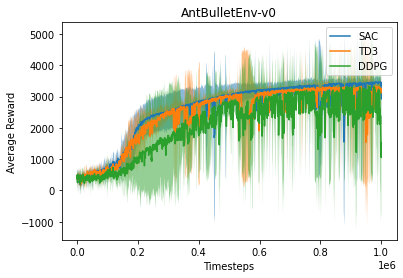
\includegraphics[width=0.45\linewidth]{photo/Ant.png}
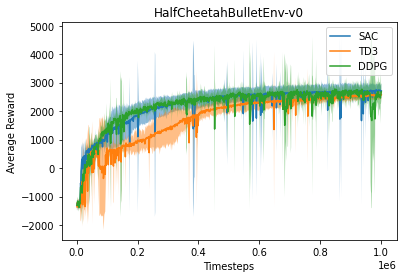
\includegraphics[width=0.45\linewidth]{photo/HalfCheetah.png}
\begin{center}
    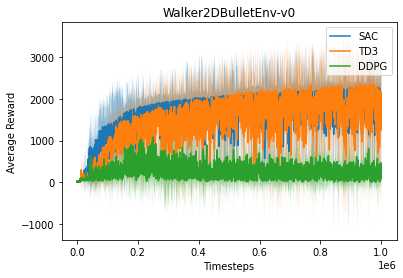
\includegraphics[width=0.45\linewidth]{photo/Walker2D.png}
\end{center}

These pictures show the average reward of three algorithm with three environment HalfCheetahBulletEnv-v0, AntBulletEnv-v0 and Walker2DBulletEnv-v0. With 4 random seed the Experiments show that SAC work very good for all of these environment. SAC and TD3 success to convert for all environment and DDPG success to convert only two of them.\\
In the AntBulletEnv-v0 environment, you can see the problem of DDPG - overestimation bias. from 200000 timesteps to 400000 timesteps the reward of DDPG is very unstable because of the problem.\\
In the HalfCheetahBulletEnv-v0 environment, DDPG is likely bester than TD3 which is realy unusual. It is because the problem of TD3 underestimation bias happen and DDPG overestimation bias problem didn't. It make the performance of DDPG bester than TD3\\
In the Walker2DBulletEnv-v0 environment, reward is very unstable. But it show that SAC work much more efficiently than the other.

\section{Future Work}
All three off-policy algorithms for continuous control we describe can be used to solve continuous control problems, but they have slow convergence and are greatly influenced by hyperparameters. We found that reinforcement learning algorithms can combine with other methods like Genetic Algorithm or Evolutionary Strategy (ES) can learn better and outperform the original deep reinforcement learning algorithms (DRL). So in the future, we want to learn about some methods that combining by ES and DRL.  

% ===================================================================================================================================
% ===================================================================================================================================


% An example of a floating figure using the graphicx package.
% Note that \label must occur AFTER (or within) \caption.
% For figures, \caption should occur after the \includegraphics.
% Note that IEEEtran v1.7 and later has special internal code that
% is designed to preserve the operation of \label within \caption
% even when the captionsoff option is in effect. However, because
% of issues like this, it may be the safest practice to put all your
% \label just after \caption rather than within \caption{}.
%
% Reminder: the "draftcls" or "draftclsnofoot", not "draft", class
% option should be used if it is desired that the figures are to be
% displayed while in draft mode.
%
%\begin{figure}[!t]
%\centering
%\includegraphics[width=2.5in]{myfigure}
% where an .eps filename suffix will be assumed under latex, 
% and a .pdf suffix will be assumed for pdflatex; or what has been declared
% via \DeclareGraphicsExtensions.
%\caption{Simulation Results}
%\label{fig_sim}
%\end{figure}

% Note that IEEE typically puts floats only at the top, even when this
% results in a large percentage of a column being occupied by floats.


% An example of a double column floating figure using two subfigures.
% (The subfig.sty package must be loaded for this to work.)
% The subfigure \label commands are set within each subfloat command, the
% \label for the overall figure must come after \caption.
% \hfil must be used as a separator to get equal spacing.
% The subfigure.sty package works much the same way, except \subfigure is
% used instead of \subfloat.
%
%\begin{figure*}[!t]
%\centerline{\subfloat[Case I]\includegraphics[width=2.5in]{subfigcase1}%
%\label{fig_first_case}}
%\hfil
%\subfloat[Case II]{\includegraphics[width=2.5in]{subfigcase2}%
%\label{fig_second_case}}}
%\caption{Simulation results}
%\label{fig_sim}
%\end{figure*}
%
% Note that often IEEE papers with subfigures do not employ subfigure
% captions (using the optional argument to \subfloat), but instead will
% reference/describe all of them (a), (b), etc., within the main caption.


% An example of a floating table. Note that, for IEEE style tables, the 
% \caption command should come BEFORE the table. Table text will default to
% \footnotesize as IEEE normally uses this smaller font for tables.
% The \label must come after \caption as always.
%
%\begin{table}[!t]
%% increase table row spacing, adjust to taste
%\renewcommand{\arraystretch}{1.3}
% if using array.sty, it might be a good idea to tweak the value of
% \extrarowheight as needed to properly center the text within the cells
%\caption{An Example of a Table}
%\label{table_example}
%\centering
%% Some packages, such as MDW tools, offer better commands for making tables
%% than the plain LaTeX2e tabular which is used here.
%\begin{tabular}{|c||c|}
%\hline
%One & Two\\
%\hline
%Three & Four\\
%\hline
%\end{tabular}
%\end{table}


% Note that IEEE does not put floats in the very first column - or typically
% anywhere on the first page for that matter. Also, in-text middle ("here")
% positioning is not used. Most IEEE journals use top floats exclusively.
% Note that, LaTeX2e, unlike IEEE journals, places footnotes above bottom
% floats. This can be corrected via the \fnbelowfloat command of the
% stfloats package.



\section{Conclusion}
In this paper, we described three off-policy algorithms for continuous control tasks. The algorithm DDPG combines the idea of DPG algorithm and the success of the DQN algorithm to expand to enable to solve tasks have high-dimensional in both action space and state space. TD3 improves the DDPG by addressing the overestimate bias problem that existed in DDPG and the first SAC version. SAC adding the entropy term in reward function and using a stochastic policy rather than a deterministic policy like DDPG and TD3 using. The Agent now need to learn how to maximize the reward and the entropy at the same time. The stochastic policy and Entropy also make the agent learn many optimal solutions for the same problem.

\section*{Acknowledgment}


%Dr. Reveryrand would like to acknowledge the funding by XLIM, Limoges, France. 
The authors would like to thank Dr. Luong Ngoc Hoang for dedicated guidance.



% if have a single appendix:
%\appendix[Proof of the Zonklar Equations]
% or
%\appendix  % for no appendix heading
% do not use \section anymore after \appendix, only \section*
% is possibly needed

% use appendices with more than one appendix
% then use \section to start each appendix
% you must declare a \section before using any
% \subsection or using \label (\appendices by itself
% starts a section numbered zero.)
%

% ============================================
%\appendices
%\section{Proof of the First Zonklar Equation}
%Appendix one text goes here %\cite{Roberg2010}.

% you can choose not to have a title for an appendix
% if you want by leaving the argument blank
%\section{}
%Appendix two text goes here.


% use section* for acknowledgement
%\section*{Acknowledgment}


%The authors would like to thank D. Root for the loan of the SWAP. The SWAP that can ONLY be usefull in Boulder...


% Can use something like this to put references on a page
% by themselves when using endfloat and the captionsoff option.
\ifCLASSOPTIONcaptionsoff
  \newpage
\fi



% trigger a \newpage just before the given reference
% number - used to balance the columns on the last page
% adjust value as needed - may need to be readjusted if
% the document is modified later
%\IEEEtriggeratref{8}
% The "triggered" command can be changed if desired:
%\IEEEtriggercmd{\enlargethispage{-5in}}

% ====== REFERENCE SECTION

%\begin{thebibliography}{1}

% IEEEabrv,

\bibliographystyle{IEEEtran}
\bibliography{IEEEabrv,Bibliography}
%\end{thebibliography}
% biography section
% 
% If you have an EPS/PDF photo (graphicx package needed) extra braces are
% needed around the contents of the optional argument to biography to prevent
% the LaTeX parser from getting confused when it sees the complicated
% \includegraphics command within an optional argument. (You could create
% your own custom macro containing the \includegraphics command to make things
% simpler here.)
%\begin{biography}[{\includegraphics[width=1in,height=1.25in,clip,keepaspectratio]{mshell}}]{Michael Shell}
% or if you just want to reserve a space for a photo:

% ==== SWITCH OFF the BIO for submission
% ==== SWITCH OFF the BIO for submission
% \begin{IEEEbiography}[{\includegraphics[width=1in,height=1.25in,clip,keepaspectratio]{photo/mike.png}}]{Michael Roberg}
% (S'09) received the B.S.E.E degree from Bucknell University, Lewisburg, PA, in 2003, the M.S.E.E. degree from the University of Pennsylvania, Philadelphia, in 2006, and the Ph.D. degree from the University of Colorado at Boulder in 2012. From 2003 to 2009, he was an Engineer with Lockheed Martin–MS2, Moorestown, NJ, where he was involved with advanced phased-array radar systems. His current research interests include high efficiency microwave PA theory and design, microwave power rectifiers, MMIC design, and high-efficiency radar and communication system transmitters. He is currently employed by TriQuint Semiconductor - Defense Products and Foundry Services in Richardson, TX working on wideband high efficiency GaN MMIC PA design.
% \end{IEEEbiography}
% \begin{IEEEbiography}[{\includegraphics[width=1in,height=1.25in,clip,keepaspectratio]{photo/tibo.png}}]{Tibault Reveyrand}
% (M'07)  received the Ph.D. degree from the University of Limoges, France, in 2002.
% From 2002 to 2004, he was a Post-Doctoral Scientist with CNES (French Space Agency). In 2005, he became a CNRS engineer at XLIM. His research interests include the characterization and modeling of RF and microwave nonlinear components and devices.
% Dr. Reveyrand was the recipient of the 2002 European GaAs Best Paper Award and is a member of the IEEE MTT-11 "Microwave Measurements" Technical Committee.
% \end{IEEEbiography}
% \begin{IEEEbiography}[{\includegraphics[width=1in,height=1.25in,clip,keepaspectratio]{photo/ignacio.png}}]{Ignacio Ramos}
% (S'12) received the B.S. degree in electrical engineering from the University of Illinois at Chicago in 2009, and is currently working toward the Ph.D. degree at the University of Colorado at Boulder. From 2009 to 2011, he was with the Power and Electronic Systems Department at Raytheon IDS, Sudbury, MA. His research interests include high-efficiency microwave power amplifiers, microwave DC/DC converters, radar systems, and wireless power transmission.
% \end{IEEEbiography}
% \begin{IEEEbiography}[{\includegraphics[width=1in,height=1.25in,clip,keepaspectratio]{photo/erez.png}}]{Erez Avigdor Falkenstein}
% (S'07), Haifa, Israel in 1979. He earned a “Handesaie” degree (associate degree) in electronics from Amal Handesaim School Hadera, Israel in 1999. From 1999 to 2003 he served in the Israel Defense Force as part of a technological unit. He has been at the University of Colorado at Boulder 2004 – 2012. He received concurrent MS/BS degrees in Electrical engineering 2010 and a Ph.D 2012 from the University of Colorado at Boulder. Since 2007 he has been involved with research as part of the active antenna group. Research emphasis: far field wireless powering for low power densities. Interests include Antenna design and characterization, modeling and measurement of nonlinear devices at microwave frequencies and power management. He is currently employed at Qualcomm, Incorporated, Boulder, CO.
% \end{IEEEbiography}
% \begin{IEEEbiography}[{\includegraphics[width=1in,height=1.25in,clip,keepaspectratio]{photo/zoya.png}}]{Zoya Popovi\'c}
% (S'86-M'90-SM'99-F'02) received the Dipl.Ing. degree from the University of Belgrade, Belgrade, Serbia, Yugoslavia, in 1985, and the Ph.D. degree from the California Institute of Technology, Pasadena, in 1990.
% Since 1990, she has been with the University of Colorado at Boulder, where she is currently a Distinguished Professor and holds the Hudson Moore Jr. Chair with the Department of Electrical, Computer and Energy Engineering. In 2001, she was a Visiting Professor with the Technical University of Munich, Munich, Germany. 
% Since 1991, she has graduated 44 Ph.D. students. Her research interests include high-efficiency, low-noise, and broadband microwave and millimeter-wave circuits, quasi-optical millimeter-wave techniques, active
% antenna arrays, and wireless powering for batteryless sensors.
% Prof. Popovi\'c was the recipient of the 1993 and 2006 Microwave Prizes presented by the IEEE Microwave Theory and Techniques Society (IEEE MTT-S) for the best journal papers and the 1996 URSI Issac Koga Gold Medal. In 1997, Eta Kappa Nu students chose her as a Professor of the Year. She was the recipient of a 2000 Humboldt Research Award for Senior U.S. Scientists of the German Alexander von Humboldt Stiftung. She was elected a Foreign Member of the Serbian Academy of Sciences and Arts in 2006. She was also the recipient of the 2001 Hewlett-Packard (HP)/American Society for Engineering Education (ASEE) Terman Medal for combined teaching and research excellence.
% \end{IEEEbiography}

%% if you will not have a photo at all:
%\begin{IEEEbiographynophoto}{Ignacio Ramos}
%(S'12) received the B.S. degree in electrical engineering from the University of Illinois at Chicago in 2009, and is currently working toward the Ph.D. degree at the University of Colorado at Boulder. From 2009 to 2011, he was with the Power and Electronic Systems Department at Raytheon IDS, Sudbury, MA. His research interests include high-efficiency microwave power amplifiers, microwave DC/DC converters, radar systems, and wireless power transmission.
%\end{IEEEbiographynophoto}
\begin{IEEEbiography}[{
\includegraphics[width=1in,height=1.25in,clip,keepaspectratio]{photo/Vu.jpg}}]{Huynh Hoang Vu}
graduated from Mac Dinh Chi High School in Ho Chi Minh City. He is studying 2rd year at University of Information Technology - VNUHCM. He belongs to the Department of Computer Science, class KHTN2020.
\end{IEEEbiography}

\begin{IEEEbiography}[{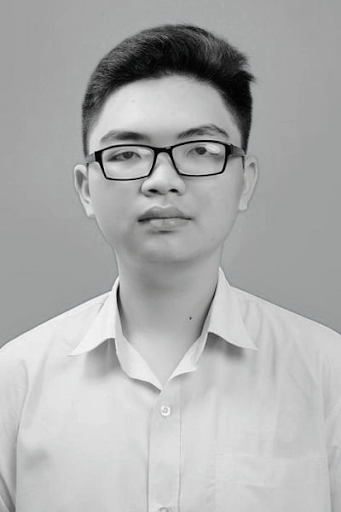
\includegraphics[width=1in,height=1.25in,clip,keepaspectratio]{photo/Luc.png}}]{Truong Mai Tan Luc}
started study a bachelor's degree at the University of Information Technology - VNUHCM, currently a second-year student in class KHTN2020 with a major in Computer Science.
\end{IEEEbiography}
\begin{IEEEbiography}[{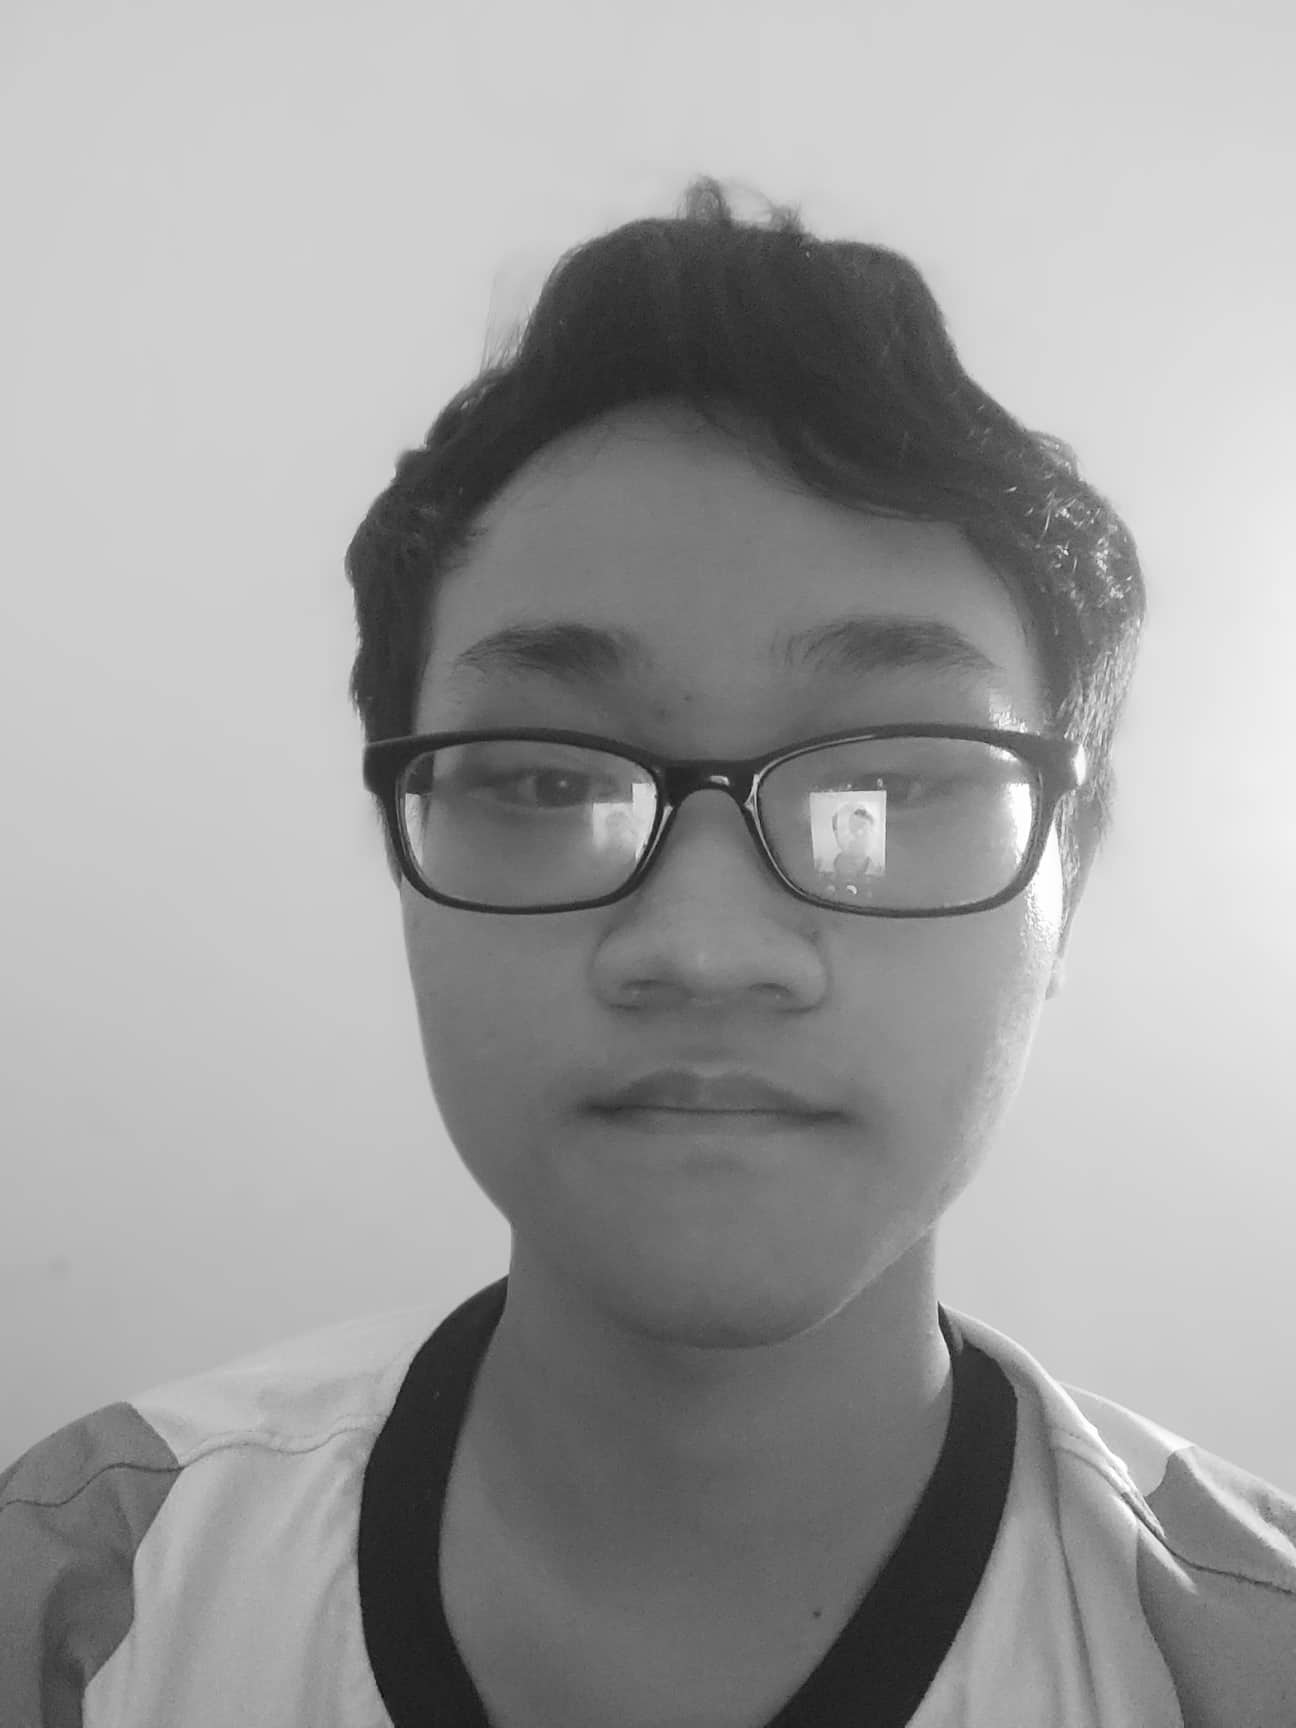
\includegraphics[width=1in,height=1.25in,clip,keepaspectratio]{photo/Khoa.png}}]{Tran Huu Khoa}
started study a bachelor's degree at the University of Information Technology - VNUHCM, currently a second-year student in class KHTN2020 with a major in Computer Science. Graduated from high school at THPT Chuyen Phan Ngoc Hien in Ca Mau
\end{IEEEbiography}


%% insert where needed to balance the two columns on the last page with
%% biographies
%%\newpage

%\begin{IEEEbiographynophoto}{Jane Doe}
%Biography text here.
%\end{IEEEbiographynophoto}
% ==== SWITCH OFF the BIO for submission
% ==== SWITCH OFF the BIO for submission



% You can push biographies down or up by placing
% a \vfill before or after them. The appropriate
% use of \vfill depends on what kind of text is
% on the last page and whether or not the columns
% are being equalized.

\vfill

% Can be used to pull up biographies so that the bottom of the last one
% is flush with the other column.
%\enlargethispage{-5in}



% that's all folks
\end{document}


